\documentclass[conference,compsoc]{IEEEtran}

% *** CITATION PACKAGES ***
%
\ifCLASSOPTIONcompsoc
  % IEEE Computer Society needs nocompress option
  % requires cite.sty v4.0 or later (November 2003)
  \usepackage[nocompress]{cite}
\else
  % normal IEEE
  \usepackage{cite}
\fi

\usepackage{graphics}
\usepackage{amsmath}
\usepackage{algorithm, algorithmic}
\renewcommand{\algorithmicrequire}{\textbf{Input:}}
\renewcommand{\algorithmicensure}{\textbf{Output:}}
\usepackage{array}
\usepackage{url}
% correct bad hyphenation here
\hyphenation{op-tical net-works semi-conduc-tor}


\begin{document}
\title{Project 4: Support Vector Machine}

% author names and affiliations
% use a multiple column layout for up to three different
% affiliations
\author{\IEEEauthorblockN{Yuejian Mo  11510511}
\IEEEauthorblockA{Department of Biology\\
Southern University of Science and Technology\\
Email: 11510511@mail.sustc.edu.cn}}

% make the title area
\maketitle

\IEEEpeerreviewmaketitle

\section{Preliminaries}
Support Vector Machine(SVM) is...
Our data ...

Support vector machine, are supervised learning models with associated learning
algorithms that analyze data used for classification and regression analysis.
Given a set of training examples, each marked as belonging to one or the other
of two categories, an SVM training algorithm builds a model that assigns new
examples to one category or the other, making it a non-probabilistic binary
linear classifier.\cite{1} If the dataset are points in space, we can find out
an gap separate dataset into two part by using SVM.

%\begin{figure}
%  \caption{Separate points into two using SVM.}
%  \centering
%    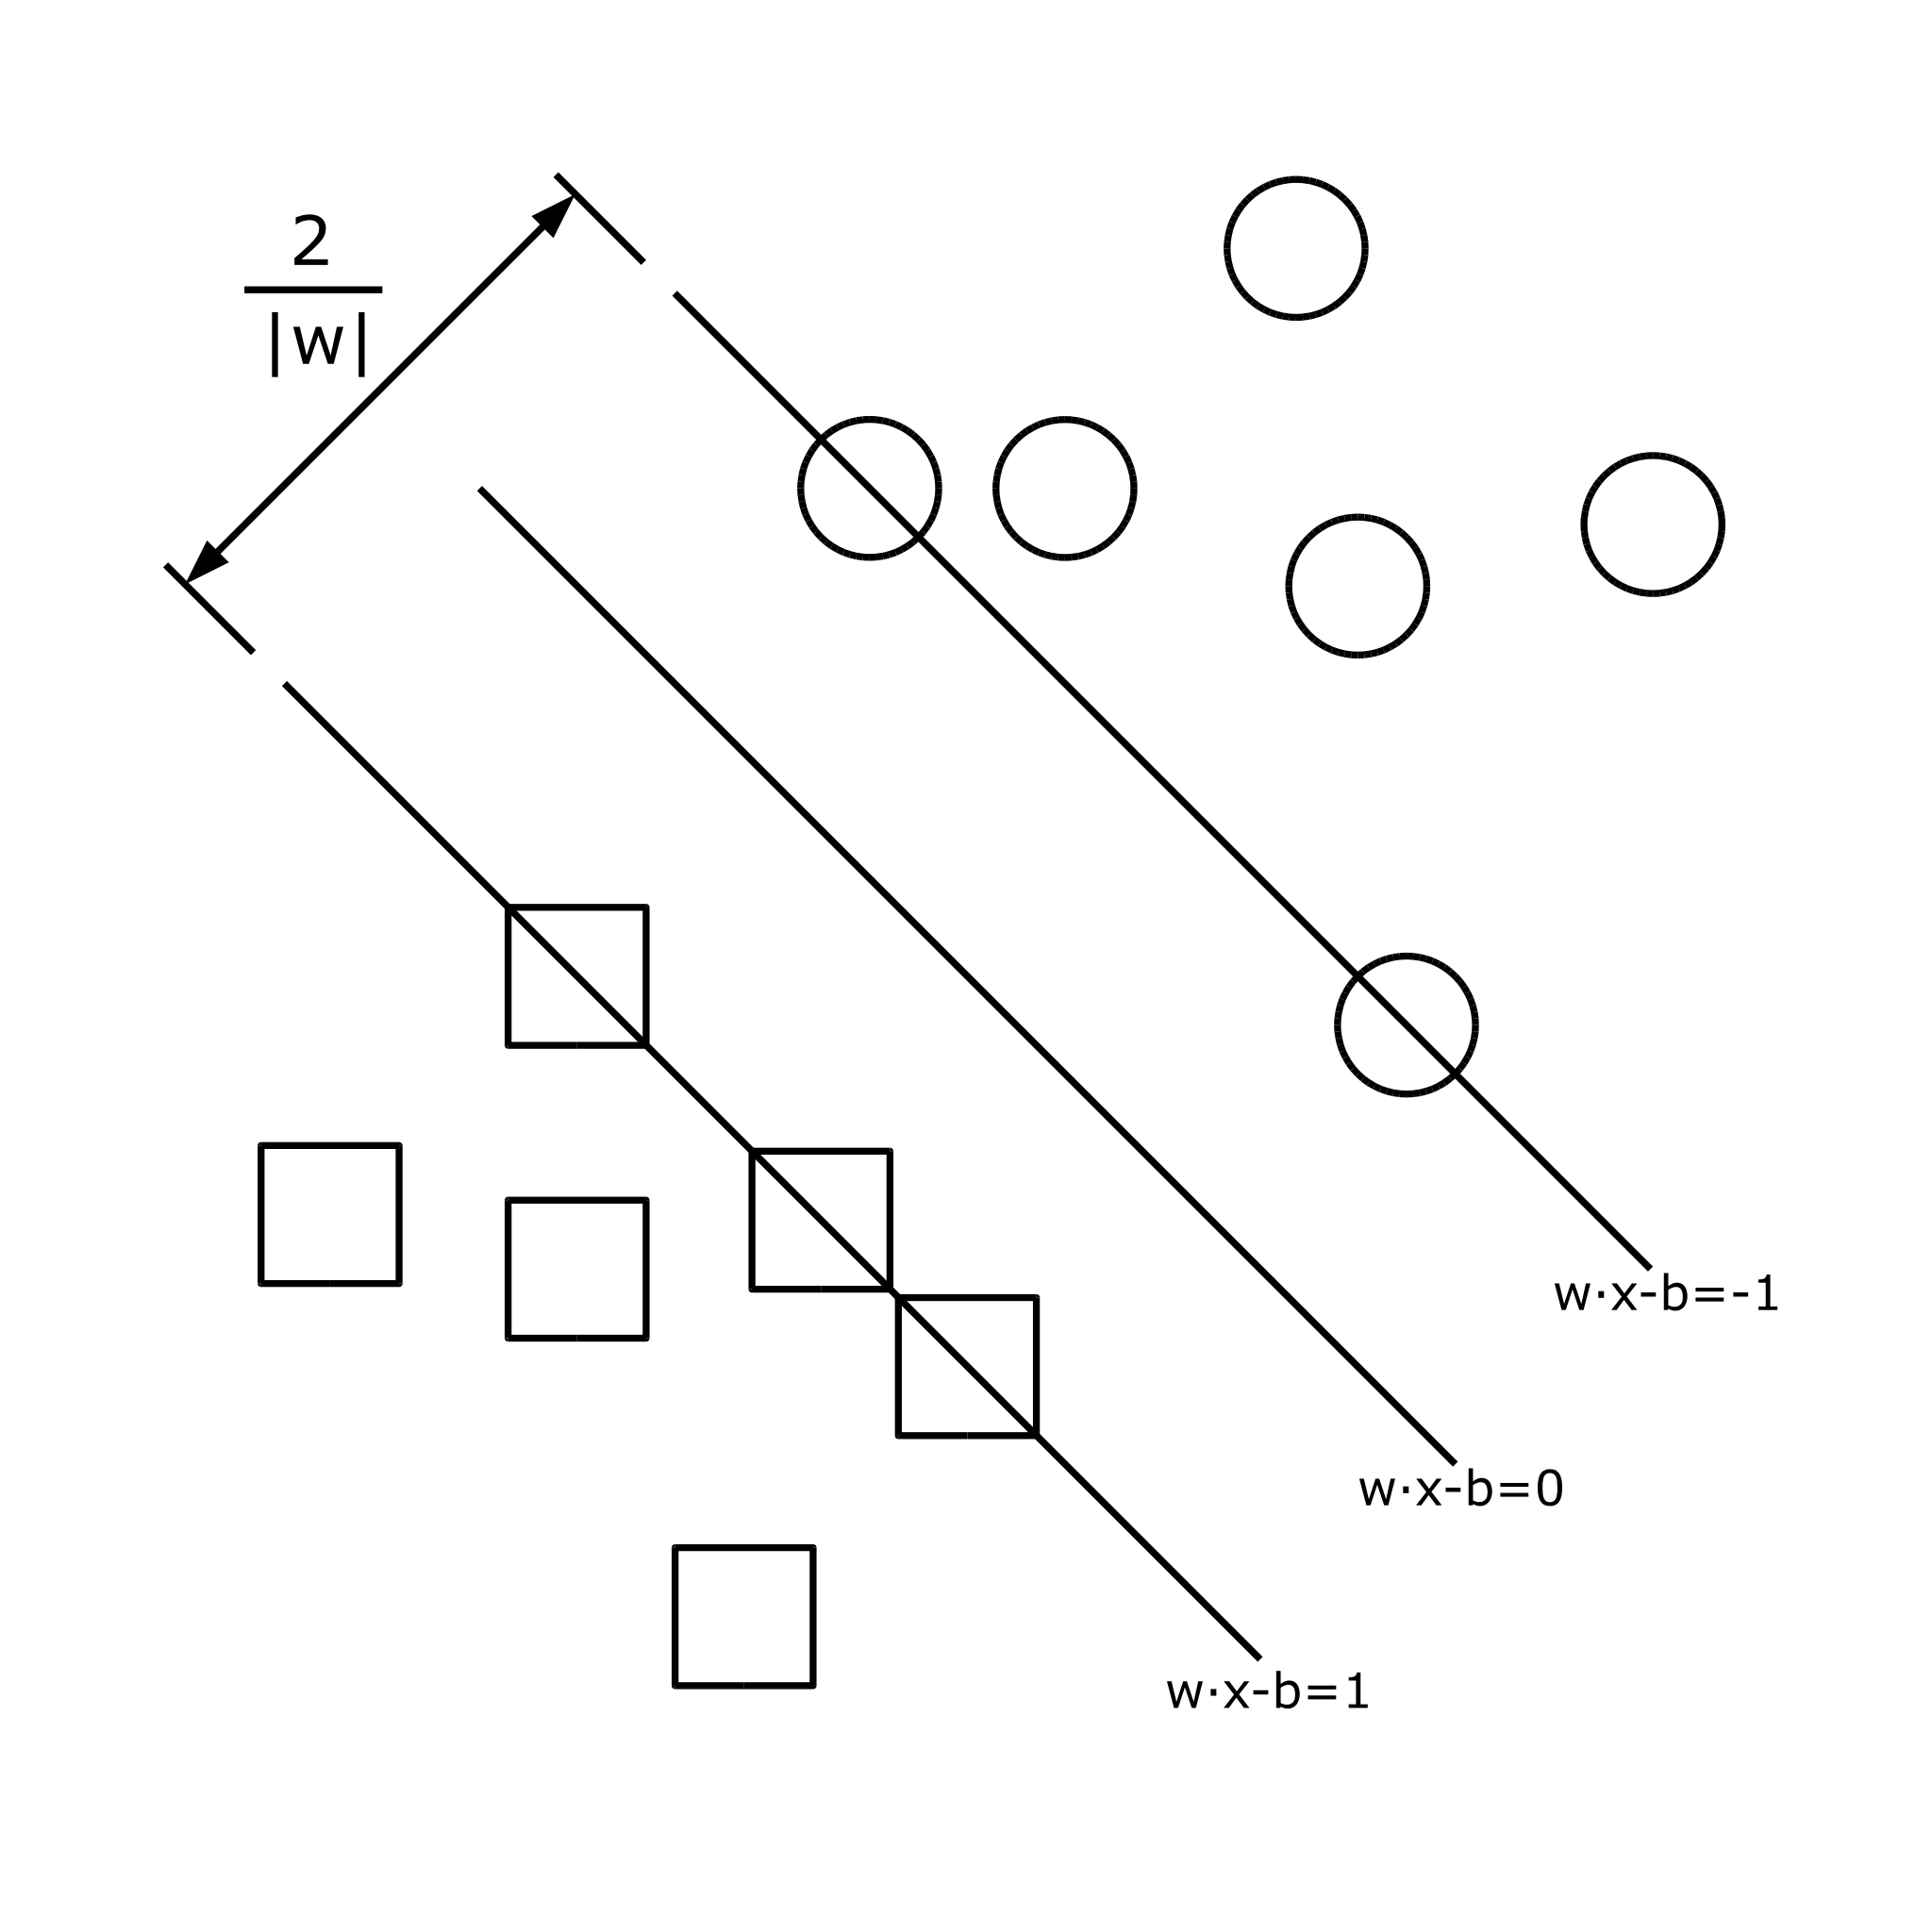
\includegraphics[width=0.5\linewidth]{SVM_margins.svg}
%\end{figure}

The original SVM algorithm was invented by Vladir N. Vapnik and
Alexey Ya. Chervonenkis in 1963. During the development, SVM are able to deal
with more tasks. SVM are used in text and hypertext categorization,
classification of images, hand-written characters recognition and proteins
classification.

In this project, I use SVM with random gradient descent to classify training
data almost correctly. 

% Add figure here

\subsection{Software}
This project is written by Python 3.7 with editor Vim. Numpy, os, time,
random, sys and argparse library are used.

\subsection{Algorithm}
Model question with SVM. To optimal time cost and current of solution, random
gradient down is used.

\section{Methodology}
Training data is ....

SVM is modeled as ...

random ....

Firstly, a social network is modeled as a directed graph $G=(V,E)$ and each
edge $(u,v)\in E$ is associated with a weight $w(u,w)=\frac{1}{d_{in}}$ which
indicates the probability that $u$ influences $v$. $S\in V$ is the subset of
nodes selected to initiate the influence diffusion,  which is called seeds set.

Then, I try to evaluate the spread influence with two different diffusion
models. In \textit{Linear Threshold} model, a node $v$ is influenced by each
neighbor $u$ according to a weight $w_{v,u}$ such that $\sum_{u}{w_{v,u}}
<=1$. The dynamics is following. Each node $v$ are accessed a threshold $\theta\in
[0,1]$ randomly obeyed uniform distribution at first step; this represents
the weighted fraction of $v$' neighbors that must become active in order
for $v$ become active. In step $t$, each inactive node $v$ will be active
by its active neighbors $w$ at step $t-1$ as following
$$\sum_{w}{w_{u,v}} >= \theta_v$$. Once no new active node is generated,
maximal spread influence will obtain with given seeds set in specified graph.
I notices final influence as the total number of active node $\sigma$.

In \textit{Independent Cascade} model, I start with an initial set of active
nodes $S$, and the process unfolds in discrete steps according to the following
randomized rule. When node $v$ first becomes active in step $t$, it is given
a single chance to activate each currently inactive neighbor $w$; it succeeds
with a probability $w_{v,w}$, independently of the history thus far. Every
step. In practical, for each inactive neighbor $w$ of new active node $v$ will
be active, if $w_{v,w}$ is larger than a new generated random number between 0 and
1 obeyed uniform distribution. (If $w$ has multiple newly activated neighbors,
their attempts are sequenced in an arbitrary order.) If $v$ succeeds, then it
cannot make any further attempts to activate $w$ in subsequent rounds. Again,
the process runs until no more activation are possible.

Both of Linear Threshold and independent Cascade model are stimulated by
repeating many time to average influence for each seed.

Finally, the seed required for IMP is generated by a natural greedy algorithm.
Each time, a node with highest influence will added to a seeds set. This empty
seed set will fill with $k$ node, where $k$ is given from outside.

\subsection{Representation}
Some main data are maintain during process: \textbf{time\_budget},
\textbf{node\_num}, \textbf{graph\_cp}, \textbf{graph\_pc}, \textbf{incoming}.
Others data would be specified inside functions.

\begin{itemize}
  \item \textbf{x}: Numpy matrix to store input data.
  \item \textbf{y}: 1-d numpy matrix of label of input data.
  \item \textbf{w}: 1-d numpy matrix of weight and bias of SVM parameters.
\end{itemize}


\subsection{Architecture}
Here list main functions of \textbf{SVM.py} in given code:
\begin{itemize}
    \item \textbf{init}: load train data to $x$, $y$; load time limit; initialize
	    parameter matrix $w$.
    \item \textbf{cal\_sgd}: Update $w$ using gradient descent.
    \item \textbf{train}: Train $w$ from train data data $x$, $y$.
    \item \textbf{predict}: Predict label of test data
    \item \textbf{\_\_main\_\_}: Main function
\end{itemize}

The \textbf{SVM.py} is executed locally.

\subsection{Detail of Algorithm}
Here describes some vital functions.
\begin{itemize}
    \item \textbf{init}: load train data and initial parameters
    \begin{algorithm}[H]
     \caption{int}
     \begin{algorithmic}[1]
     \renewcommand{\algorithmicrequire}{\textbf{Input:}}
     \renewcommand{\algorithmicensure}{\textbf{Output:}}
     \REQUIRE $input\_file\_name, time\_limit$
     \ENSURE $x, y, w, cycle$
     \STATE open $input\_file\_name$ as $file$ \COMMENT{open file and read line
     by line}
     \STATE \COMMENT{Read each line information until arrive edge information}
     \STATE set $data$
     \FOR {each line in $file$}
          \STATE split line, then package and append line info to $data$
     \ENDFOR
     \STATE transform set $data$ to matrix $x$
     \STATE $y \leftarrow x[:,-1]$ 
     \STATE $x[:, -1] \leftarrow 1$
     \STATE initialize $w$ with length of $x[:, -1]$ and value of 0
     \STATE $cycle$
     \RETURN $x, y, w, cycle$
     \end{algorithmic}
   \end{algorithm}

   \item \textbf{cal\_sgd}:Update $w$ using gradient descent
     \begin{algorithm}[H]
     \caption{cal\_sgd}
     \begin{algorithmic}[2]
     \renewcommand{\algorithmicrequire}{\textbf{Input:}}
     \renewcommand{\algorithmicensure}{\textbf{Output:}}
     \REQUIRE $xi, yi, w, ratio, learn\_speed$
     \ENSURE $w\_next$ 
     \IF {$yi*(\cdot{xi}{w}) < 1$}
	     \STATE $w\_next = w - ratio*(learn\_speed*w - yi*xi)$
     \ELSE
	     \STATE $w\_next = w - ratio*learn\_speed*yi$
     \ENDIF
     \RETURN $w\_next$
     \end{algorithmic}
     \end{algorithm}

  \item \textbf{train}: Train $w$ with data $x, y$
    \begin{algorithm}[H]
     \caption{train}
     \begin{algorithmic}[3]
     \renewcommand{\algorithmicrequire}{\textbf{Input:}}
     \renewcommand{\algorithmicensure}{\textbf{Output:}}
     \REQUIRE $x, y, w, cnt, learn\_speed$
     \ENSURE  $w$
     \STATE $t \leftarrow 0$
     \WHILE{ running time don't exceed ordered time}
	     \STATE reorder $x$ and $x$ in the same time
	     \STATE $loss \leftarrow 0$ 
	     \STATE $t \leftarrow t+1$
	     \STATE $1//(t*learn\_speed)$
	     \FOR{ each line $x_i$ and $y_i$ in training data}
	          \STATE $w = cal\_sgd(x_i, y_i, w, ratio, learn\_speed$
	     \ENDFOR
     \ENDWHILE
     \RETURN $w$
     \end{algorithmic}
     \end{algorithm}
 
 \item \textbf{hill\_greedy}: Generate optimal seed using Hill Greedy Algorithm
     \begin{algorithm}[H]
     \caption{hill\_greedy}
     \begin{algorithmic}[4]
     \renewcommand{\algorithmicrequire}{\textbf{Input:}}
     \renewcommand{\algorithmicensure}{\textbf{Output:}}
     \REQUIRE $size, model$
     \ENSURE  $seeds$
     \STATE create empty $ans\_seeds$
     \STATE $cnt \leftarrow 0$
     \WHILE{$cnt \ne size$}
	\STATE copy $ans\_seeds$ to $cur\_seed$
	\STATE $high \leftarrow 0$
	\STATE $point \leftarrow 1$
        \FOR{each node $4$ don't be chosen}
	     \STATE add $v$ to $cur\_seed$
	     \IF{$model$ == IC}
	          \STATE $new\_high \leftarrow IC(graph\_pc,cur\_speed, incoming)$ 
	     \ELSE
	          \STATE $new\_high \leftarrow LT(graph\_cp,cur\_speed, incoming)$ 
	     \ENDIF
	     \IF{$nw\_high \le high$}
	         \STATE $high \leftarrow new\_high$
		 \STATE $point \leftarrow v$
	     \ENDIF
        \ENDFOR
	\STATE add $point$ to $ans\_seeds$
	\STATE $cnt \leftarrow cnt+1$
     \ENDWHILE
     \RETURN $ans\_seeds$
     \end{algorithmic}
     \end{algorithm}
 

\end{itemize}


\section{Empirical Verification}
Empirical verification is confirmed in OJ system. $ISE.py$ almost pass all
dataset with reasonable bias. $IMP.py$ only was test with network-5-IC and
provide reasonable seeds set.

\subsection{Design}
SVM classify data at less 90 percent robust.

Random gradient return in reasonable time than simple gradient down algorithm.

Independent cascade model return reasonable influence is small graph and big graph.
But Linear Threshold model return less reasonable due with large graph. Finally,
I found my code would added some element repeatedly result in larger bias.

For hill greedy, because I just evaluate once, it produce seeds set fast. In
small graph, which produce seeds in 65 percent effect. But
Not optimal seeds are produced every time.

\subsection{Data and data structure}
Dictionaries and lists are used widely rather than matrix. Because the input graph
is sparse, dictionary are always used to store graph as adjacent list. Global
variable $graph\_pc$, $graph\_cp$ and $incoming$ are dictionary. Lists always
store routes and edges information for local variable.

\subsection{Performance}
Following table show different performance with different dataset. Offline
test perform at Fedora 29 with $Intel^{®}$ Xeon(R) CPU E5-1680 v3@3.20GHz and
32GiB memory.

\begin{center}
   \begin{tabular}{| l | l | l |}
   \hline
    Dataset             &Run Time(s)   &Result   \\ \hline
    network-seeds-IC     & 23.23        & 5.015  \\
    network-seeds-LT     & 23.23        & 5.015  \\
    network-seeds2-IC    & 23.24        & 30.47  \\ 
    network-seeds2-LT    & 57.79        & 37.03  \\
    NetHEPT-5seeds-LT    & 58.55        & 341.9  \\
    NetHEPT-5seeds-IC    & 27.87        & 276.3  \\
    NetHEPT-50seeds-LT    &         &   \\
    NetHEPT-50seeds-IC    & 27.87        & 1003  \\
    network-5-IC         & 0.73         & 19.45  \\
   \hline
   \end{tabular}
\end{center}
% Table of difference problem

\subsection{Result}
% 
Solutions are accepted most all public dataset' test. But Linear Threshold model
produce influence with large bias. 

\subsection{Analysis}
% Analysis different parameter's results
Because natural Hill Greedy is kind of greedy algorithm without heuristics, most
of solutions are not optimal. During using adjacent list rather than adjacent
matrix, space cost is more lower than $O(n^2)$. Because every point only is
evaluate once, only less time it cost. Total, no more than $O(n^2)$ is required.

\section*{Acknowledgment}
Thanks TA Yao Zhao who explain question and provide general method to solve it.
And I also thanks for Kebing Sun discuss and share the idea about algorithm.

\bibliographystyle{IEEEtran}
\begin{thebibliography}{1}
\bibitem{1}
Kempe D, Kleinberg J, Tardos É. Maximizing the spread of influence through a
social network[C]//Proceedings of the ninth ACM SIGKDD international conference
on Knowledge discovery and data mining. ACM, 2003: 137-146.

\end{thebibliography}

% that's all folks
\end{document}


